\section{Structuration et programmation}

Quand j'étais arrivée, la structure de codes et celle de \db\ étaient définies par Ophir. Au début, j'ai continué avec celles d'Ophir, mais après le dégagement développement, les structures étaient changés. Dans ce chapitre, je vais montrer les changements structurels de \db\ et de codes, aussi des réalisations codage de certains parties de la plate-forme.

\subsection{Structuration de \db\ }

La \db\ était structurée selon la conception qui demande à garder tous les livres et layers dedans

\begin{figure}[H]
\centering
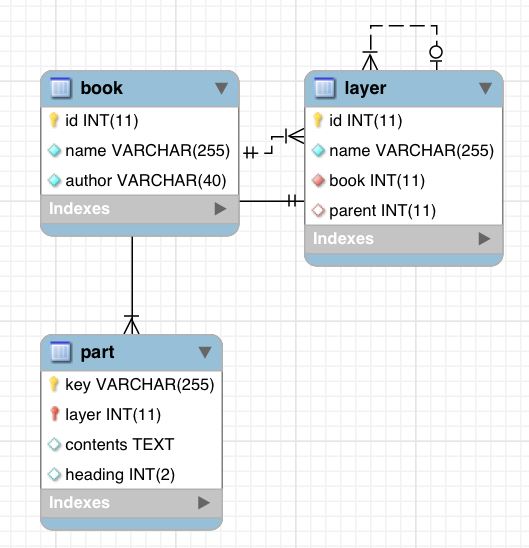
\includegraphics[width=\textwidth]{ancienne_structure}
\caption{L'ancienne structure de \db\ }
\end{figure}

\subsection{Structuration de codes}

\subsection{Réalisation d'édition de transcription}

\subsection{Réalisation d'accès}

\subsection{Réalisation de la gestion de groups}